\documentclass[12pt]{article}

\usepackage{amsmath}
\usepackage{graphicx}
\usepackage{hyperref}

\title{Your Report Title}
\author{Your Name}
\date{\today}

\begin{document}

\maketitle

\begin{abstract}
This is the abstract of your report. It should provide a brief summary of the content and main findings of the report.
\end{abstract}

\section{Introduction}
This is the introduction section. Here you should introduce the topic of your report, provide some background information, and state the objectives of your work.

\section{Linear SVM }

This section discusses the hyperparameter tuning and results of a linear support vector machine implementation. 

\subsection{Optimal Tuning}
This model was tuned using K-fold Cross Validation and several values of C, the regularization parameter CHECK THIS SHIT. 
To find the optimal value of C, the following format was used B > 1 and C0 > 0 with C = C0 raised to the B * ith power where i is the iteration number. The optimal value for C with the lowest average loss for kfold validation where k = 10 with 2000 data points sampled from the original 12000 was 2.2 * 10^4 or 22193 or 1.1 ** 7*15.

\begin{figure}
    \centering
    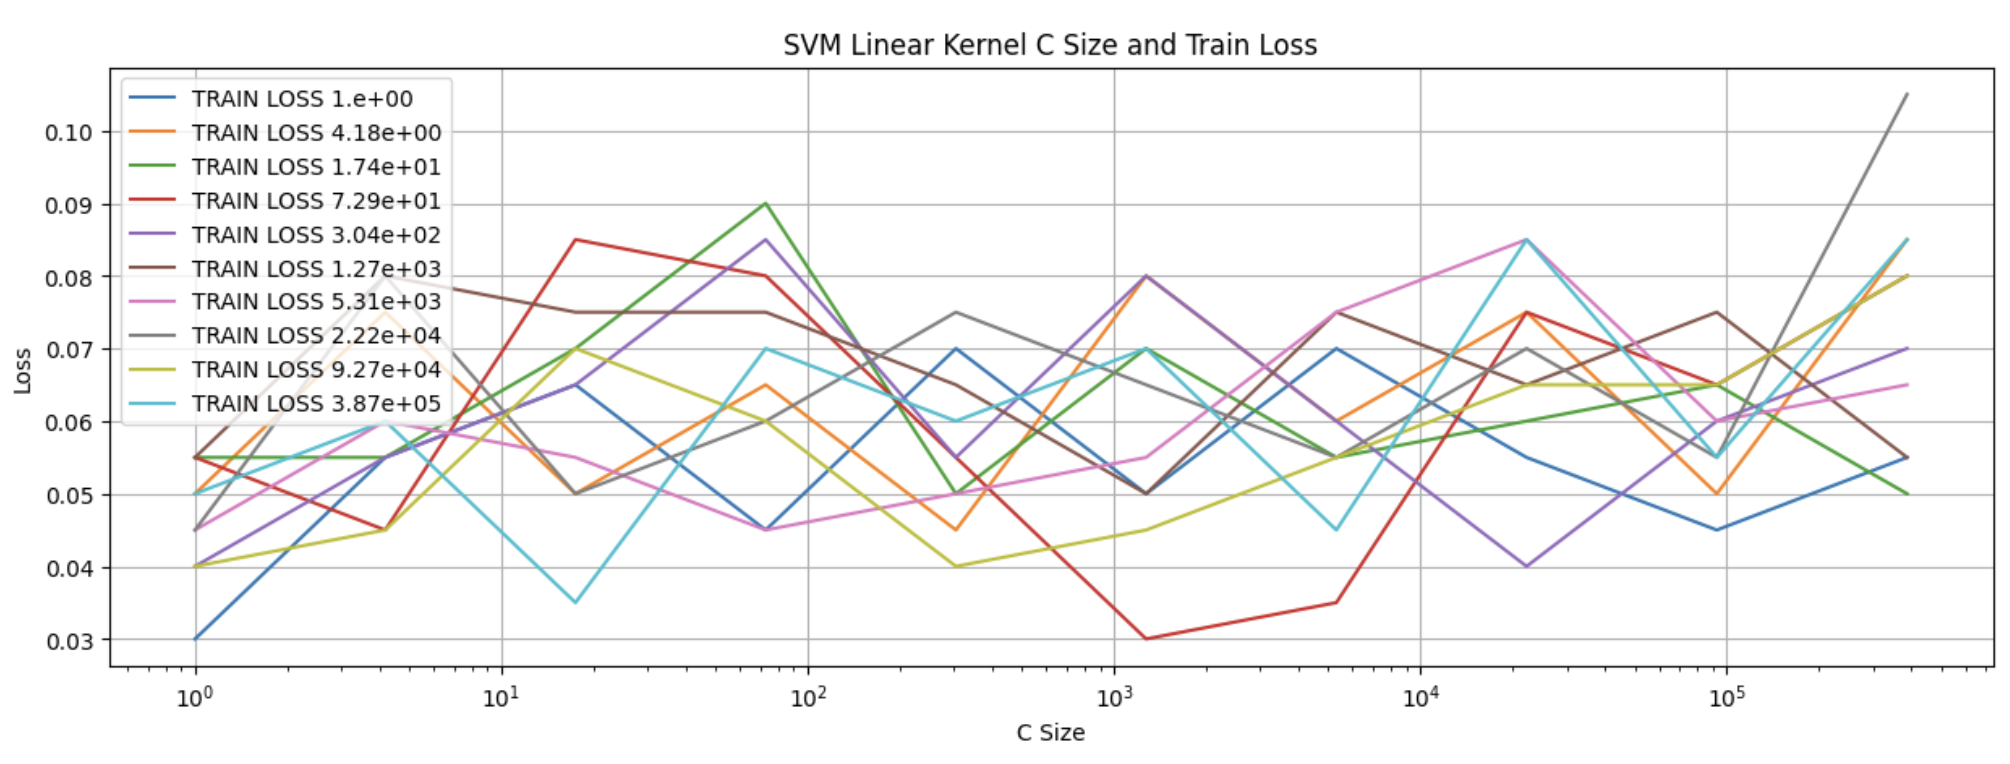
\includegraphics{Assets/LinearSVM_TrainLosses.png}
    \caption{Linear SVM Training Losses}
\end{figure}

\subsection{Total Train and Test Loss}

BLAH BLAH BLAH RESULTS THAT TAKE A LONG TIME TO COMPUTE




\section{Kernelized SVM}
This section should describe the methods and procedures you used in your work. Be sure to provide enough detail so that someone else could replicate your study.

\section{Neural Network}
Here you should present the results of your work. This can include tables, figures, and descriptive text.

\section{Model Comparison}
In this section, you should interpret your results and discuss their implications. You can also discuss any limitations of your study and suggest areas for future research.

\section{Conclusion}
This is the conclusion section. Summarize the main findings of your report and restate the significance of your work.


\end{document}